\subsection{Overview}
This section goes over how the S\&C platform will be implemented and tested. Through testing it is possible to identify and correct possible bugs proactively, greatly decreasing the risk of a user having problems while using Students\&Companies. In the following sections it will be described how the system will be implemented and how its components will be tested.

\subsection{Testing and Implementation Plan}
The system will be tested and implemented using a bottom-up approach, incrementally adding components as their dependencies are fully tested and integrated. This means that every component will be using its actual dependencies and will be activated by drivers that simulate the behaviour of the upstream components. This testing flow has the advantage of being straightforward and easy to adopt since it reduces the number of mock components that must be created and many components have the same dependencies hence they can be tested simultaneously, speeding up the implementation process.
\\
\begin{figure}[h]
    \centering
    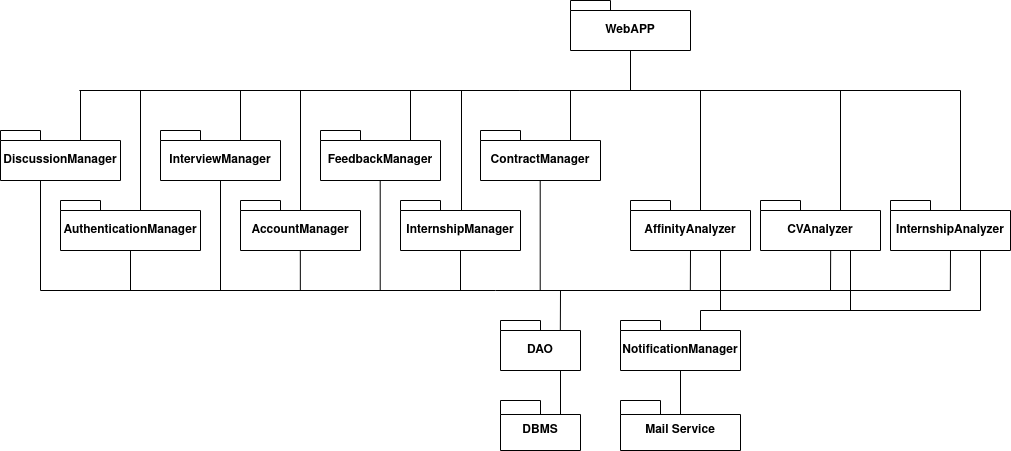
\includegraphics[width=1\linewidth]{Images/testing.drawio(1).png}
    \caption{Dependencies of the components}
    \label{fig:compdep}
\end{figure}
\\
In figure \ref{fig:compdep} are represented by the dependencies between components. Using the bottom-up approach means that for example, the analyzers will be tested after the testing of DAO and NotificationManager is completed. To test the WebAPP component the REST API will be used to submit requests and check that the responses are correct and no errors occur.

\subsection{Additional System Testing}
After the system is fully implemented, there are other aspects which can be tested to ensure that the platform is able to guarantee non-functional requirements such as availability, security and response times. To check this aspects the following tests can be done:
\begin{itemize}
    \item \textbf{Performance testing}: a basic test in which requests are submitted simulating the expected load. This can be used to ensure that everything works as expected under normal conditions, resulting in a positive user experience, and to identify possible bottlenecks or inefficiencies.
    \item \textbf{Stress testing}: there is a possibility of the system receiving more requests than expected. By generating an artificially high number of requests it will be tested if the system is able to handle them or, in the eventuality of crashes due to the high load, is able to gracefully recover.
    \item \textbf{Security testing}: this test is aimed at finding possible vulnerabilities on the platform. This is performed by checking that malicious requests are successfully rejected.
\end{itemize}